\documentclass[10pt,onecolumn]{book}

\usepackage{times} % font
\usepackage{graphicx} % picture reference
\usepackage{amsmath} % split of mathematical formulas
\usepackage{amssymb} % special mathematical symbols
\usepackage{geometry} % margin
\usepackage{setspace} % letter-spacing
\usepackage{indentfirst} % indent
\geometry{left=2cm,right=2cm, top=2cm, bottom=2cm}
\usepackage{hyperref} % hyperlink
\usepackage{cite}
\usepackage[sectionbib]{chapterbib}

\usepackage{multirow}
\usepackage{color}
\usepackage{ulem}
\usepackage{todonotes}

%\usepackage{fancy}%页眉页脚包
%\pagestyle{plain}%页眉页脚设置
\usepackage{fancyhdr}
\pagestyle{fancy}


\def\ie{\emph{i.e.}}
\def\eg{\emph{e.g.}}
\def\etal{\em {et al.}}

\newcommand{\bm}[1]{\mbox{\boldmath{$#1$}}}
\newcommand{\figref}[1]{Fig. \ref{#1}}
\newcommand{\tabref}[1]{Tab. \ref{#1}}
\newcommand{\equref}[1]{(\ref{#1})}
\newcommand{\secref}[1]{Sect. \ref{#1}}
\newcommand{\algref}[1]{Alg. \ref{#1}}
\newcommand{\myPara}[1]{\vspace{.05in}\noindent\textbf{#1}}
\newcommand{\rev}[1]{\textcolor{blue}{#1}}
\newcommand{\rr}[1]{\textcolor{red}{#1}}
\newcommand{\cg}[1]{\textcolor{green}{#1}}
\newcommand{\bb}[1]{\textcolor{blue}{#1}}
\newcommand{\bl}[1]{\textbf{#1}}
\newcommand{\ul}[1]{\underline{#1}}
\newcommand{\mc}[1]{\mathcal{#1}}
\newcommand{\mb}[1]{\mathbb{#1}}

\begin{document}

\title{\textbf{Paper Reading}}
\author{Jinming Su}
\date{Last update: \today}

\maketitle

\thispagestyle{empty}
\newpage
\pagenumbering{Roman}
\newpage
\tableofcontents
%\newpage
%\listoffigures
%\newpage
%\listoftables
%\newpage
%\pagenumbering{arabic}
\newpage
\listoftodos

\newpage
\pagenumbering{arabic}
\mainmatter

\chapter{Classification}
\section{Res2Net: A New Multi-scale Backbone Architecture, arxiv, 2019.}
\begin{figure}[h]
\centering
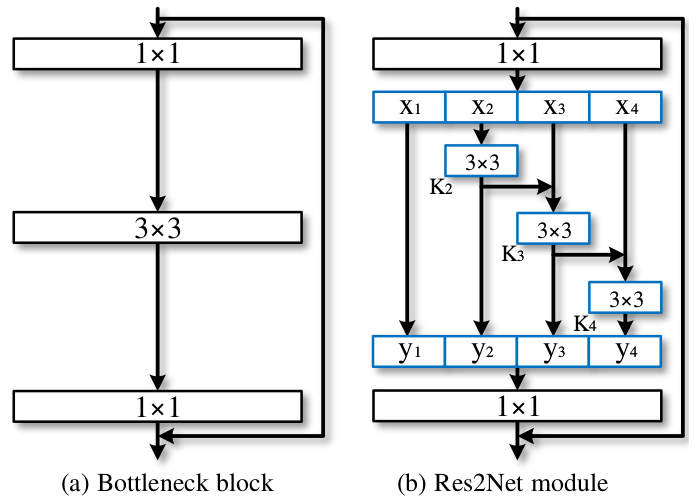
\includegraphics[width=0.4\textwidth]{figures_paper_reading/Res2Net:_A_New_Multi-scale_Backbone_Architecture.png}
\caption{Residual Learning.}
\label{fig:1-1_residual_learning}
\end{figure}
This paper is mainly a promotion of residual network, which seems to be similar to cardinality, only adding more connections.

\chapter{Salient Object Detection}
\section{DNA: Deeply-supervised Nonlinear Aggregation for Salient Object Detection. arxiv, 2019.}
\begin{figure}[h]
\centering
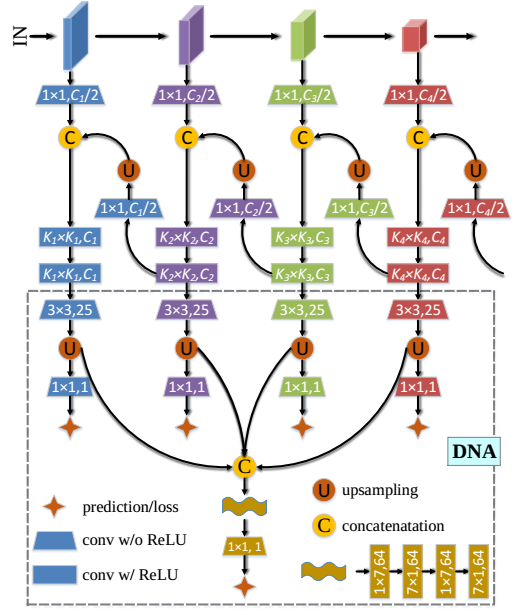
\includegraphics[width=0.4\textwidth]{figures_paper_reading/DNA_Deeply-supervised_Nonlinear_Aggregation_for_Salient_Object_Detection.png}
\caption{Residual Learning.}
\label{fig:1-1_residual_learning}
\end{figure}

This paper has two contributions: 
(1) \uline{theoretically and experimentally} analyzes the natural limitaion of traditional side-output aggregration which can only make limited use of multi-scale side-ouput informantion; 
(2) proposes Deeply-supervised nonlinear aggregration (DNA) for side-output features. 
(3) as experience, in DNA, convolution layers with kernels of $n \times 1$ and $1 \times n$ are used, which is proved to be effective. Moreover, authers claim that large kernel size in DNA can improve performance.

\chapter{Object Detection}
\section{Proposal}
\subsection{Multiscale Combinatorial Grouping for Image Segmentation and Object Proposal Generation. TPAMI, 2016}
I don't read this paper, but the code is tested. Code can be found in \url{https://github.com/jponttuset/mcg}. When testing, run pre-trained/install.m, pre-trained/demos/demo\_im2mcg.m and get the following results.
\begin{figure}[h]
\centering
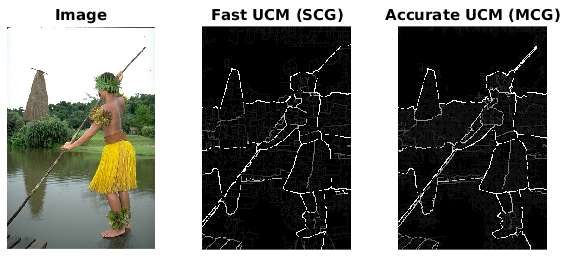
\includegraphics[width=0.6\textwidth]{figures_paper_reading/MCG_UCM.png}
\caption{The UCM of MCG.}
\label{fig}
\end{figure}

\begin{figure}[h]
\centering
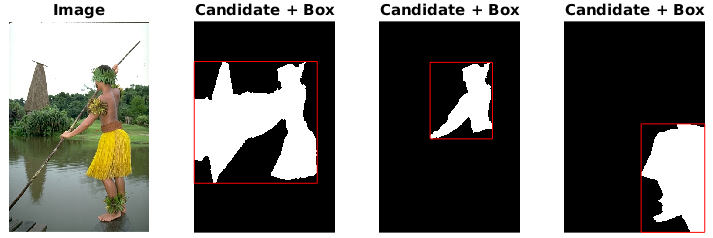
\includegraphics[width=0.8\textwidth]{figures_paper_reading/MCG.png}
\caption{The results of MCG.}
\label{fig}
\end{figure}

\section{What Object Should I Use? - Task Driven Object Detection. CVPR, 2019.}
\begin{figure}[h]
\centering
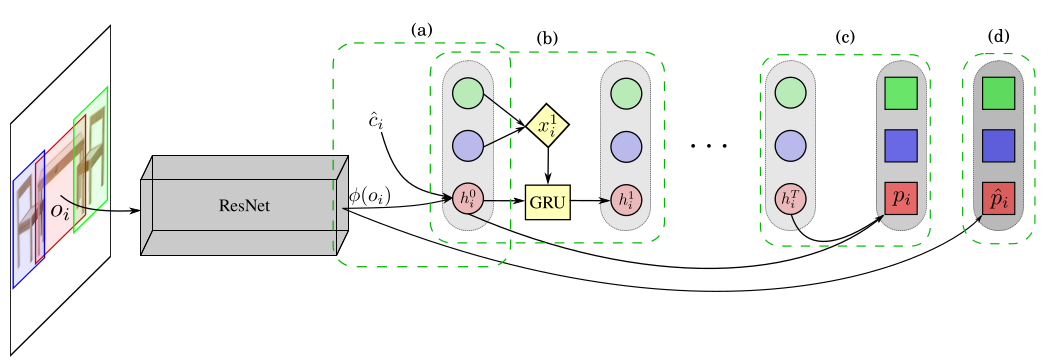
\includegraphics[width=0.8\textwidth]{figures_paper_reading/What_Object_Should_I_Use?_-_Task_Driven_Object_Detection.png}
\caption{GGNN.}
\label{fig}
\end{figure}

This paper has two contributions:
(1) construct a COCO-Tasks dataset which comprises about 40,000 images where the most suitable objects for 14 \uline{tasks} have been annotated;
(2) proposes a method buliding on \uline{Gated Graph Neural Network} to detect the most suitable objects for a given task. 

\chapter{Semantic Segmentation}
\begin{figure}[h]
\centering
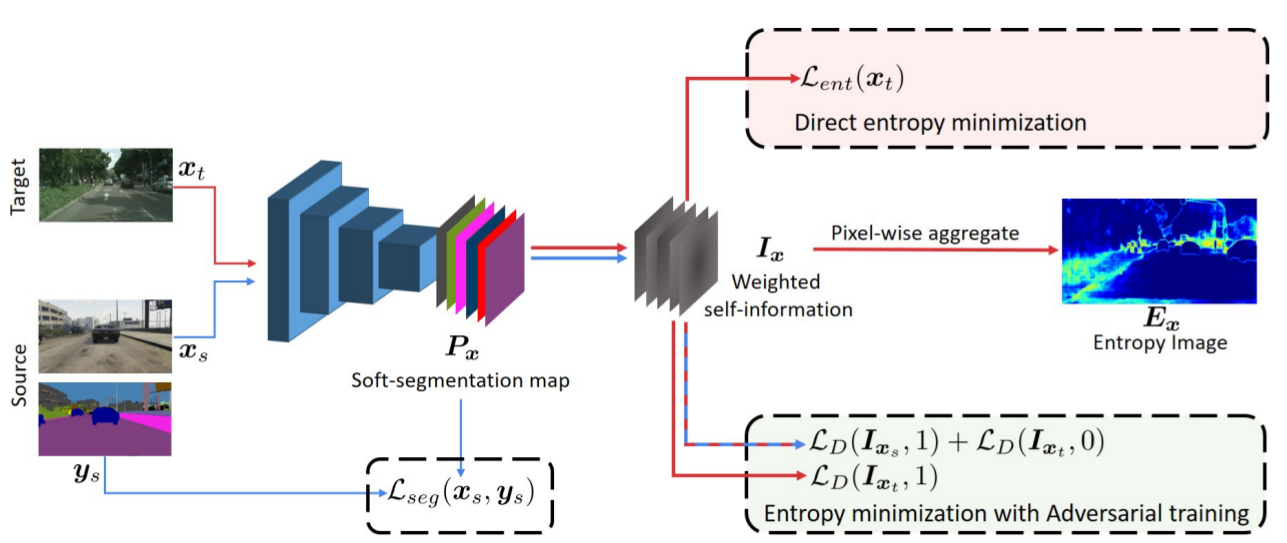
\includegraphics[width=0.8\textwidth]{figures_paper_reading/ADVENT_Adversarial_Entropy_Minimization_for_Domain_Adaptation_in_Semantic_Segmentation_CVPR2019.png}
\caption{Advsarial entropy.}
\label{fig}
\end{figure}
This paper focuses on the problem of domain adapation in semantic segmentation. In detail, the contributions are as follows: (1) propose to minimize the pixel-level entropy of target domain to penalize low-confident predictions on target domain; (2) propose a entropy-based adversarial traing approach to privide the structure adaptation; (3) extra two trick: a) training on specific entropy ranges and b) add class-ratio priors.

\chapter{Others}
\section{Single Image Haze Removal Using Dark Channel Prior. CVPR, 2009. Best paper.}
This paper introduces dark channel prior that is an observation -most local patches in haze-free outdoor images contain some pixels which have very low intensities in at least one color channel. \uline{This is the one of most famous papers in the domain of dehazing.} 

Some formulas in this paper are easy to understand. One can refer to \url{https://www.cnblogs.com/Imageshop/p/3281703.html} for more understanding. 

The unofficial python code can be found in \url{https://github.com/su526664687/dark-channel-prior-dehazing}.

\section{Single Image Dehazing Using Ranking Convolutional Neural Network. TMM, 2018.}
\begin{figure}[h]
\centering
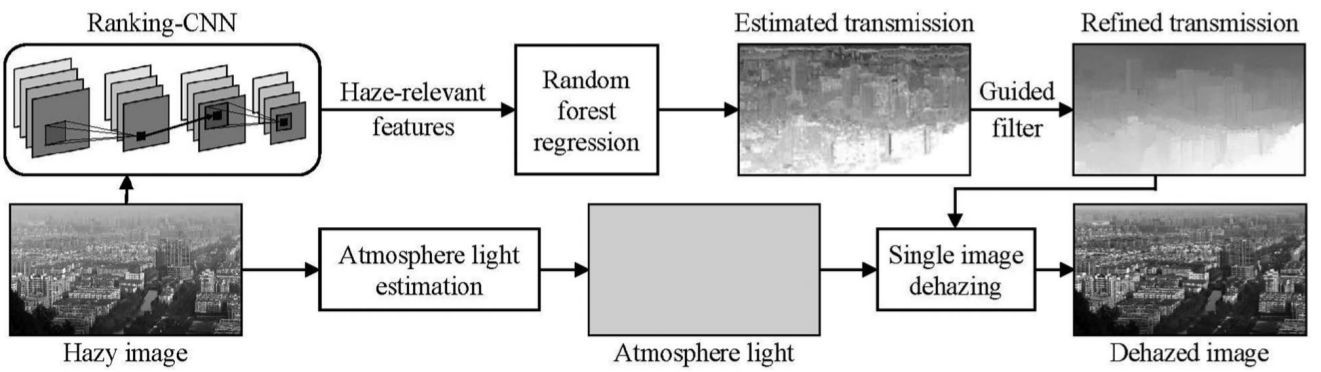
\includegraphics[width=0.8\textwidth]{figures_paper_reading/Single_Image_Dehazing_Using_Ranking_Convolutional_Neural_Network.png}
\caption{GGNN.}
\label{fig}
\end{figure}

This paper presents a ranking cnn to deal with dehazing. The ranking-cnn mainly means a ranking layer. In this layer, the values in a feature map are ranked, and the same operation is conducted for each feature map. Moreover, this paper introduce a method to synthesize haze images.

~\cite{su2019for}

{\small
\bibliographystyle{plain}
\bibliography{Ref_paper_reading}
}

\end{document}
